\documentclass[sigconf]{acmart}

% ---------------------------------------------------------------
% IMPORTANT: This document requires the ACM acmart template.
% Download acmart.cls and ACM-Reference-Format.bst from:
%   https://www.acm.org/publications/proceedings-template
% Place those two files in the same directory as this .tex file,
% then compile with: pdflatex -> bibtex -> pdflatex -> pdflatex
% Alternatively, upload to Overleaf using the ACM SigConf template.
% ---------------------------------------------------------------

\usepackage{booktabs}
\usepackage{multirow}
\graphicspath{{../results/}}

% Remove ACM reference block and copyright footer for draft submission
\settopmatter{printacmref=false}
\renewcommand\footnotetextcopyrightpermission[1]{}
\setcopyright{none}
\acmConference[FPCC2 2026]{Fundamentos de Pesquisa Cient\'{i}fica em Computa\c{c}\~{a}o}{2026}{UFCG, Brazil}
\acmYear{2026}
\acmDOI{}
\acmISBN{}

% ---------------------------------------------------------------
\begin{document}

\title{Reproducing Confidential LLM Inference: A Performance Study of CPU Trusted Execution Environments}

\author{Raisson Adrian Grangeiro Souto}
\affiliation{%
  \institution{Universidade Federal de Campina Grande}
  \city{Campina Grande}
  \state{Para\'{i}ba}
  \country{Brazil}
}
\email{raisson.souto@copin.ufcg.edu.br}

% ---------------------------------------------------------------
\begin{abstract}
Large Language Models (LLMs) are increasingly deployed on cloud infrastructure where
they process sensitive and proprietary data, raising significant concerns about model
intellectual property theft and user data confidentiality. Trusted Execution Environments
(TEEs) have emerged as a practical mechanism for end-to-end confidential LLM inference,
offering hardware-enforced memory isolation with manageable performance overhead. This
paper presents a reproduction study of Chrapek et al.~\cite{chrapek2025confidential},
which originally characterized LLM inference performance and cost across CPU and GPU
TEEs. We focus on reproducing the CPU TEE results for the Llama2 7B model, comparing
Intel Software Guard Extensions (SGX) via the Gramine library OS and Intel Trust Domain
Extensions (TDX) against a conventional virtual machine (VM) baseline. Our experimental
design is multifactorial with 30 repetitions per configuration, varying batch sizes
(1 and 64) and input sequence lengths (128, 512, and 2048 tokens), with Advanced
Matrix Extensions (AMX) acceleration disabled to isolate the overhead contribution of
the TEE mechanism itself. The central claim under examination is whether CPU TEEs impose
less than 10\% throughput overhead on LLM inference, and whether this bound holds on
hardware distinct from the original study's Intel Xeon platforms.
\end{abstract}

% ---------------------------------------------------------------
\begin{CCSXML}
<ccs2012>
 <concept>
  <concept_id>10002978.10003006.10011747</concept_id>
  <concept_desc>Security and privacy~Trusted computing bases</concept_desc>
  <concept_significance>500</concept_significance>
 </concept>
 <concept>
  <concept_id>10010147.10010257</concept_id>
  <concept_desc>Computing methodologies~Machine learning</concept_desc>
  <concept_significance>300</concept_significance>
 </concept>
 <concept>
  <concept_id>10002951.10003227.10003351</concept_id>
  <concept_desc>Information systems~Cloud computing</concept_desc>
  <concept_significance>300</concept_significance>
 </concept>
</ccs2012>
\end{CCSXML}

\ccsdesc[500]{Security and privacy~Trusted computing bases}
\ccsdesc[300]{Computing methodologies~Machine learning}
\ccsdesc[300]{Information systems~Cloud computing}

\keywords{Confidential Computing; Trusted Execution Environments; Large Language Models;
Intel SGX; Intel TDX}

\maketitle

% ---------------------------------------------------------------
\section{Introduction}

Large Language Models (LLMs) have become essential infrastructure across industries
ranging from healthcare to financial analysis~\cite{llm_survey}, yet their computational
demands make on-premises deployment impractical for most organizations. LLM workloads
are consequently migrated to Cloud Service Providers, where they routinely handle
sensitive data: patient records, confidential legal documents, and proprietary financial
analyses~\cite{chrapek2025confidential}. This exposes them to threats from malicious
insiders, adversarial co-tenants, and compromised hypervisors, with breaches carrying
severe financial consequences given that model training costs can reach tens of millions
of dollars~\cite{chrapek2025confidential}.

The security research community has explored three primary classes of protection mechanisms
for LLM deployments in adversarial cloud environments. \emph{Machine learning-based
methods}, including model watermarking and ownership
verification schemes, operate post-hoc, detecting IP theft after it has occurred rather
than actively preventing unauthorized access. These methods also fail to protect the
confidentiality of user prompts. \emph{Cryptographic methods}, such as Homomorphic
Encryption (HE)~\cite{he_ml} and Secure Multi-Party Computation (MPC), provide strong
provable security guarantees but impose performance overheads of up to four orders of
magnitude, making them intractable for the compute-intensive inference workloads of modern
LLMs. \emph{Confidential Computing} via Trusted Execution Environments (TEEs) addresses
both limitations: it actively enforces trust boundaries through hardware isolation and
provides cryptographic attestation, with overheads substantially lower than cryptographic
alternatives~\cite{tee_ml_survey}.

TEEs establish a \emph{secure enclave}, a hardware-protected memory region inaccessible
to the operating system, hypervisor, or co-tenants, and support \emph{remote attestation},
allowing remote parties to verify the integrity and authenticity of the executing software.
Two dominant strategies exist for CPU-based TEEs in cloud deployments. \emph{Process-based
TEEs}, exemplified by Intel Software Guard Extensions (SGX)~\cite{intel_sgx}, protect
individual processes within an encrypted Enclave Page Cache (EPC), with overhead arising
from EPC paging, enclave transitions, and memory integrity verification. \emph{VM-based
TEEs}, exemplified by Intel Trust Domain Extensions (TDX)~\cite{intel_tdx}, protect an
entire virtual machine using a hardened KVM hypervisor, offering a broader trust boundary
and simpler deployment at the cost of an additional virtualization performance penalty.

Chrapek et al.~\cite{chrapek2025confidential} conducted the first comprehensive study of
LLM inference performance and cost across both CPU and GPU TEEs. Their evaluation runs full
Llama2 (7B, 13B, 70B) inference pipelines within Intel SGX and TDX on two Intel Xeon
server platforms, using Intel Extension for PyTorch (IPEX)~\cite{ipex} as the
best-performing inference framework. A complementary GPU TEE evaluation is conducted on
an NVIDIA H100 NVL instance from Microsoft Azure. From this evaluation, the authors
derive 12 key insights. Among the most significant: CPU TEEs impose throughput overheads
below 10\% and latency overheads below 20\%, further mitigated by Advanced Matrix
Extensions (AMX) acceleration. TDX is considerably easier to deploy than SGX but incurs
a higher virtualization tax of 1--5\% on top of the baseline overhead, and for small LLMs
at low batch sizes, CPU TEEs can be more cost-effective than confidential GPU
counterparts.

Reproducibility is a cornerstone of scientific progress, yet systems research results
are frequently sensitive to hardware microarchitecture, software versions, and
infrastructure configuration. This paper reproduces the findings of
Chrapek et al.~\cite{chrapek2025confidential} on independent hardware, using their
released artifacts,\footnote{\url{https://github.com/spcl/confidential-llms-in-tees}}
to assess whether the reported overhead bounds generalize beyond the specific platforms
of the original study. The evaluation compares Intel SGX via the Gramine library OS and
Intel TDX against a conventional VM baseline for Llama2 7B, across batch sizes of 1 and
64 and input lengths of 128, 512, and 2048 tokens, with 30 repetitions per configuration.

\subsection{Research Questions}
\label{sec:rqs}

This reproduction study is guided by the following research questions:

\begin{itemize}
  \item \textbf{RQ1:} Do CPU TEEs (Intel SGX, Intel TDX) impose less than 10\%
  throughput overhead relative to a non-TEE VM baseline for Llama2 7B inference on
  independent hardware?
  \item \textbf{RQ2:} Does the relative throughput/latency overhead of CPU TEEs
  diminish as batch size and input sequence length increase?
\end{itemize}

RQ1 tests whether the original study's central overhead bound generalizes to hardware
distinct from the Intel Xeon platforms used by Chrapek et al. RQ2 tests whether the
overhead-amortization trend reported in the original work reproduces in this
environment. Section~\ref{sec:methodology} describes the experimental methodology, and
Section~\ref{sec:results} reports how the collected evidence answers RQ1 and RQ2.

% ---------------------------------------------------------------
\section{Methodology}
\label{sec:methodology}

\subsection{Scope}
\label{sec:scope}

This study re-executes the experiment of Chrapek et al.~\cite{chrapek2025confidential}
using their released codebase, focusing on CPU TEE results for \textbf{Llama2 7B}~\cite{llama2}
across three execution environments: a conventional VM (baseline), Intel SGX via
Gramine~\cite{gramine}, and Intel TDX. GPU TEE experiments are not reproduced, as the
CPU results constitute the primary empirical contribution of the original study. Batch
sizes of 1 and 64 and input lengths of 128, 512, and 2048 tokens are selected to span
the behavioral regimes identified in the original work. AMX acceleration is disabled
throughout to isolate baseline TEE overhead, and all experiments use bfloat16 precision.

\subsection{Experimental Design}

The study follows a \textbf{multifactorial design} across execution environment, batch
size, and input sequence length. Table~\ref{tab:factors} summarizes the factors and levels.

\begin{table}[t]
  \caption{Experimental factors and their levels.}
  \label{tab:factors}
  \begin{tabular}{ll}
    \toprule
    \textbf{Factor} & \textbf{Levels} \\
    \midrule
    Execution environment & VM (baseline), SGX, TDX \\
    Batch size            & 1, 64 \\
    Input sequence length & 128, 512, 2048 tokens \\
    \bottomrule
  \end{tabular}
\end{table}

This yields $3 \times 2 \times 3 = 18$ configurations, each with \textbf{30 independent
repetitions} ($540$ runs total). Output length is fixed at 128 tokens with greedy
decoding. Overheads are computed relative to the VM baseline within each factor combination.

\textbf{Independent variables:} execution environment (VM, SGX, TDX), batch size (1, 64),
and input sequence length (128, 512, 2048 tokens).

\textbf{Dependent variables:} throughput (tokens/s), next-token latency (ms), CPU
utilization (\%), peak memory utilization (GB), and estimated cloud cost (\$/million
tokens). Medians across repetitions are reported for all metrics.

These variables directly instrument the two research questions from
Section~\ref{sec:rqs}: throughput and latency, expressed as overhead relative to the VM
baseline, instrument \textbf{RQ1}; their variation across the batch-size and
input-length factor levels instruments \textbf{RQ2}.

\subsection{Infrastructure and Software Stack}

All environments run on Linux VMs with 16 vCPUs, 64\,GB RAM, and Ubuntu 24.04 LTS,
provisioned via Scontain confidential computing infrastructure or Microsoft Azure. The software stack follows the original
study~\cite{chrapek2025confidential}: IPEX~\cite{ipex}~2.x for inference, PyTorch~2.x
with Hugging Face Transformers~4.x for model loading, Gramine~\cite{gramine} as the SGX
runtime, and TCMalloc as the memory allocator. Llama2 7B is loaded in bfloat16 without
quantization, with synthetic workloads generating at least 1,000 output tokens per
repetition to obtain stable throughput estimates.

\subsection{Differences from the Original Study}

Table~\ref{tab:differences} summarizes the main differences between the original study
and this reproduction. The narrower scope reflects resource availability rather than
methodological disagreement; the selected configurations are sufficient to evaluate the
original study's central performance claims.

\begin{table*}[t]
  \caption{Comparison between the original study and this reproduction.}
  \label{tab:differences}
  \small
  \begin{tabular}{p{3.2cm} p{6cm} p{6cm}}
    \toprule
    \textbf{Aspect} & \textbf{Original Study} & \textbf{This Reproduction} \\
    \midrule
    Models & Llama2 7B/13B/70B, Llama3 8B, Mistral 7B, Gemma 7B & Llama2 7B only \\
    \midrule
    Execution environments & Bare metal, VM, Intel SGX, Intel TDX, NVIDIA H100 cGPU &
                             VM (baseline), Intel SGX, Intel TDX (no bare metal, no GPU TEE) \\
    \midrule
    Batch sizes & 1--512 & 1, 64 \\
    \midrule
    Input lengths & 32--2048 tokens & 128, 512, 2048 tokens \\
    \midrule
    AMX acceleration & Enabled and disabled (comparative analysis) & Disabled only \\
    \midrule
    Data types & bfloat16 and int8 & bfloat16 only \\
    \midrule
    Hardware & Intel Xeon Gold 6530 (32 cores) and Intel Xeon Platinum 8580 (60 cores) &
               Intel-compatible VM, 16 vCPUs, 64\,GB RAM \\
    \midrule
    Repetitions & Not specified & 30 per configuration \\
    \midrule
    GPU TEE evaluation & NVIDIA H100 NVL (Azure, $\approx$\$30K/month) & Not included \\
    \bottomrule
  \end{tabular}
\end{table*}

Results and analysis are presented in the subsequent sections.

% ---------------------------------------------------------------
\section{Results and Discussion}
\label{sec:results}

The measurement matrix described in Section~\ref{sec:methodology} has been executed on
the Azure confidential-computing VMs: 13 of the 18 configurations completed all 30
repetitions and were parsed into the consolidated CSV published with the artifacts
(Section~\ref{sec:reproducibility}). The five missing cells are batch-64 runs with
512-token (SGX, TDX) and 2048-token (all three environments) inputs, which were killed
by out-of-memory conditions --- inside the SGX enclave
(\texttt{DefaultCPUAllocator: can't allocate memory}) and by the host OOM killer for
the baseline and TDX arms. Figures~\ref{fig:batch-scaling}, \ref{fig:overhead-trend},
\ref{fig:cost-batches}, and~\ref{fig:cost-inputs} present the collected data.
\textbf{[PLACEHOLDER]} Table~\ref{tab:overhead} and the interpretation paragraphs below
remain to be finalized from the CSV.

\subsection{Throughput and Latency Overhead (RQ1)}
\label{sec:results-rq1}

Table~\ref{tab:overhead} reports, for each of the 18 configurations (3 execution
environments $\times$ 2 batch sizes $\times$ 3 input lengths, 30 repetitions each), the
median throughput, median next-token latency, and the resulting overhead relative to
the VM baseline within the same batch size/input length cell.
Figure~\ref{fig:batch-scaling} shows the median throughput and relative overhead at
128-token inputs --- the only input length at which all three environments completed
both batch sizes.

\begin{figure}[t]
  \centering
  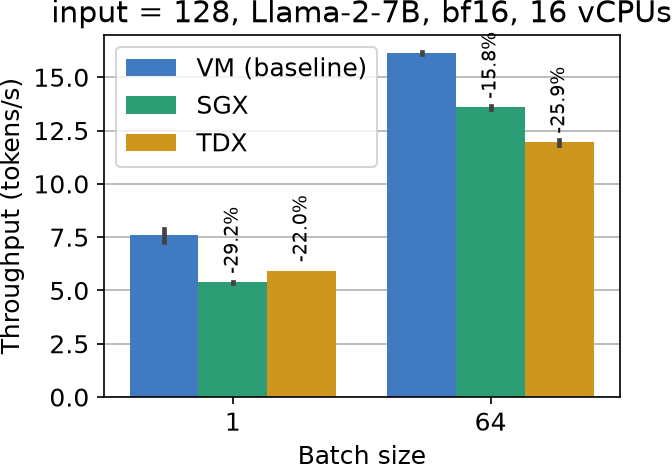
\includegraphics[width=\linewidth]{batch_scaling_combined.png}
  \caption{Median throughput at 128-token inputs, by batch size and execution
  environment (30 repetitions; error bars span the observed range). Labels give the
  throughput reduction of SGX and TDX relative to the VM baseline.}
  \label{fig:batch-scaling}
\end{figure}

\begin{table*}[t]
  \caption{Median throughput, latency, and overhead relative to the VM baseline, by
  configuration (\textbf{TBD}: pending experiment execution).}
  \label{tab:overhead}
  \small
  \begin{tabular}{llccccc}
    \toprule
    \textbf{Environment} & \textbf{Batch} & \textbf{Input (tok)} & \textbf{Throughput (tok/s)} & \textbf{Latency (ms)} & \textbf{Overhead (\%)} \\
    \midrule
    \multirow{6}{*}{VM (baseline)} & \multirow{3}{*}{1}  & 128  & TBD & TBD & --- \\
                                    &                     & 512  & TBD & TBD & --- \\
                                    &                     & 2048 & TBD & TBD & --- \\
                                    & \multirow{3}{*}{64} & 128  & TBD & TBD & --- \\
                                    &                     & 512  & TBD & TBD & --- \\
                                    &                     & 2048 & TBD & TBD & --- \\
    \midrule
    \multirow{6}{*}{SGX (Gramine)}  & \multirow{3}{*}{1}  & 128  & TBD & TBD & TBD \\
                                    &                     & 512  & TBD & TBD & TBD \\
                                    &                     & 2048 & TBD & TBD & TBD \\
                                    & \multirow{3}{*}{64} & 128  & TBD & TBD & TBD \\
                                    &                     & 512  & TBD & TBD & TBD \\
                                    &                     & 2048 & TBD & TBD & TBD \\
    \midrule
    \multirow{6}{*}{TDX}            & \multirow{3}{*}{1}  & 128  & TBD & TBD & TBD \\
                                    &                     & 512  & TBD & TBD & TBD \\
                                    &                     & 2048 & TBD & TBD & TBD \\
                                    & \multirow{3}{*}{64} & 128  & TBD & TBD & TBD \\
                                    &                     & 512  & TBD & TBD & TBD \\
                                    &                     & 2048 & TBD & TBD & TBD \\
    \bottomrule
  \end{tabular}
\end{table*}

\textbf{[PLACEHOLDER --- RQ1 interpretation]} Once populated, this paragraph will state
whether the overhead column in Table~\ref{tab:overhead} stays below the 10\% bound
reported by Chrapek et al.~\cite{chrapek2025confidential} for both Intel SGX and Intel
TDX on this reproduction's hardware, or whether it exceeds that bound, directly
answering RQ1.

\subsection{Effect of Batch Size and Input Length (RQ2)}
\label{sec:results-rq2}

\begin{figure*}[t]
  \centering
  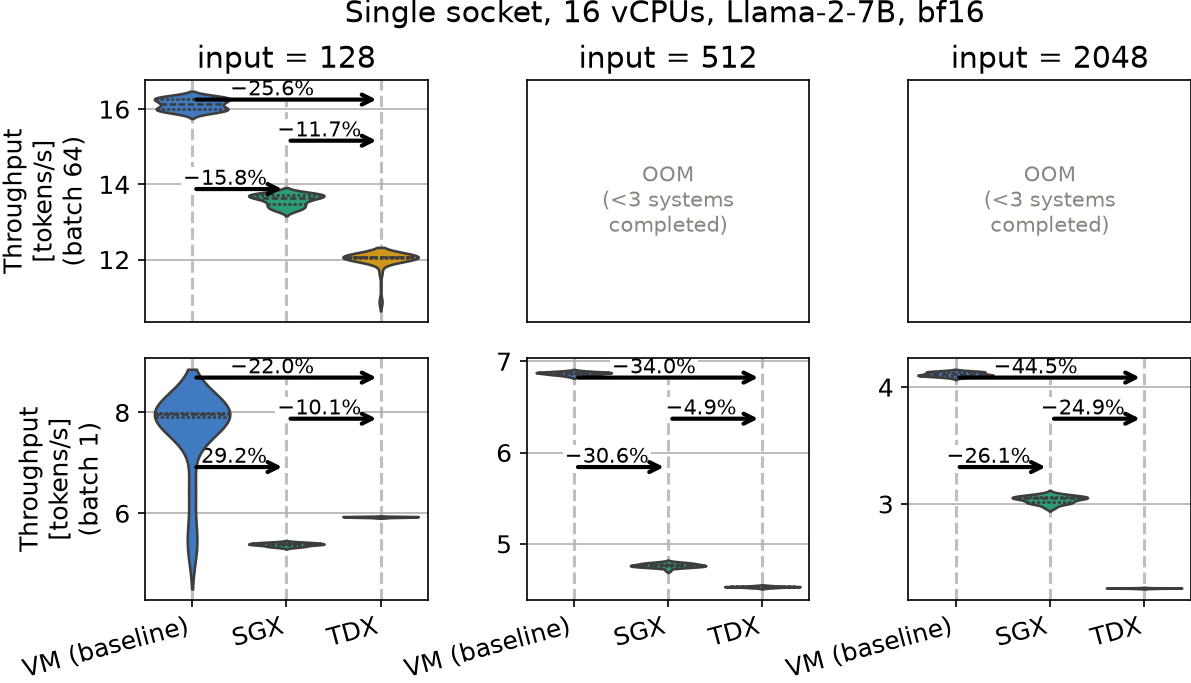
\includegraphics[width=0.92\textwidth]{overall_single_socket.png}
  \caption{Throughput distributions over 30 repetitions for each execution environment,
  input length (columns), and batch size (rows). Annotations give median relative
  throughput differences between environments. Batch-64 panels at 512 and 2048 input
  tokens are marked OOM: fewer than three environments completed
  (Section~\ref{sec:results}).}
  \label{fig:overhead-trend}
\end{figure*}

Figure~\ref{fig:overhead-trend} shows the throughput distributions across the full
factor space, generated from the consolidated CSV by the scripts in
\texttt{CPU/processing/}.

\textbf{[PLACEHOLDER --- RQ2 interpretation]} Once populated, this paragraph will state
whether Figure~\ref{fig:overhead-trend} shows the overhead-amortization trend reported
in the original study --- i.e., relative overhead shrinking as batch size and input
length grow --- or whether the trend does not reproduce on this hardware, directly
answering RQ2.

\subsection{Estimated Cost}
\label{sec:results-cost}

\begin{figure}[t]
  \centering
  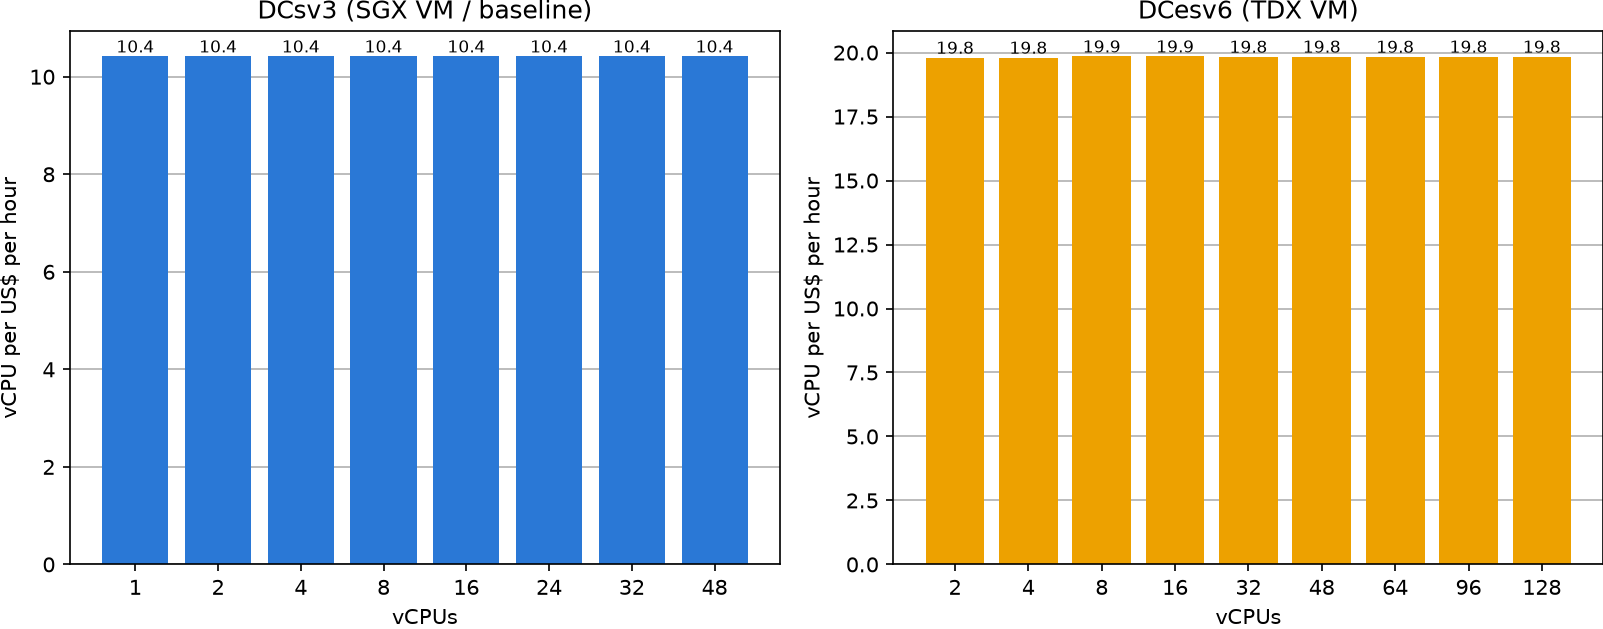
\includegraphics[width=\linewidth]{azure_price.png}
  \caption{Azure pay-as-you-go pricing efficiency (vCPUs per US\$ per hour) of the two
  VM families used, fetched from the Azure Retail Prices API: DCsv3 (baseline and SGX
  arms) and DCesv6 (TDX arm).}
  \label{fig:azure-price}
\end{figure}

\begin{figure}[t]
  \centering
  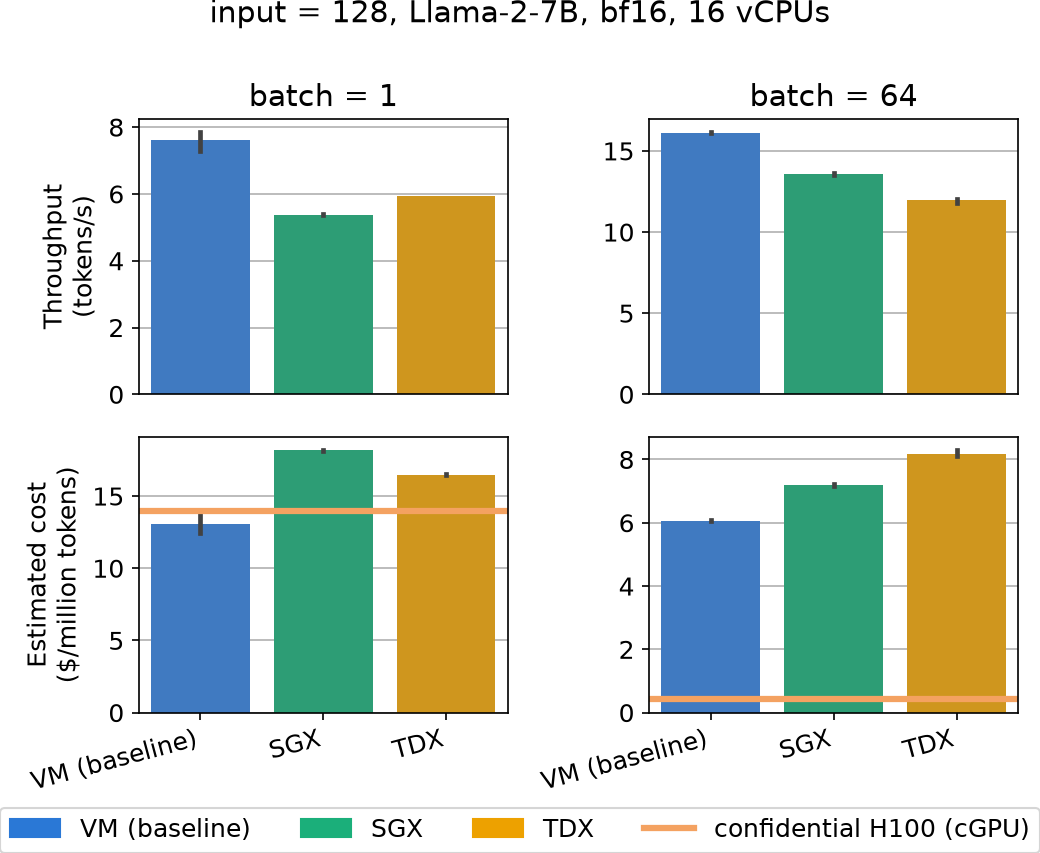
\includegraphics[width=\linewidth]{vCPUs_GPU_EMR_batches.png}
  \caption{Measured throughput (top) and estimated cost per million generated tokens
  (bottom) at 128-token inputs, by batch size, using the original artifact's Azure cost
  model (per-vCPU and per-GB-of-RAM hourly rates). The horizontal line is the
  confidential H100 (cGPU) estimate from the same model.}
  \label{fig:cost-batches}
\end{figure}

\begin{figure*}[t]
  \centering
  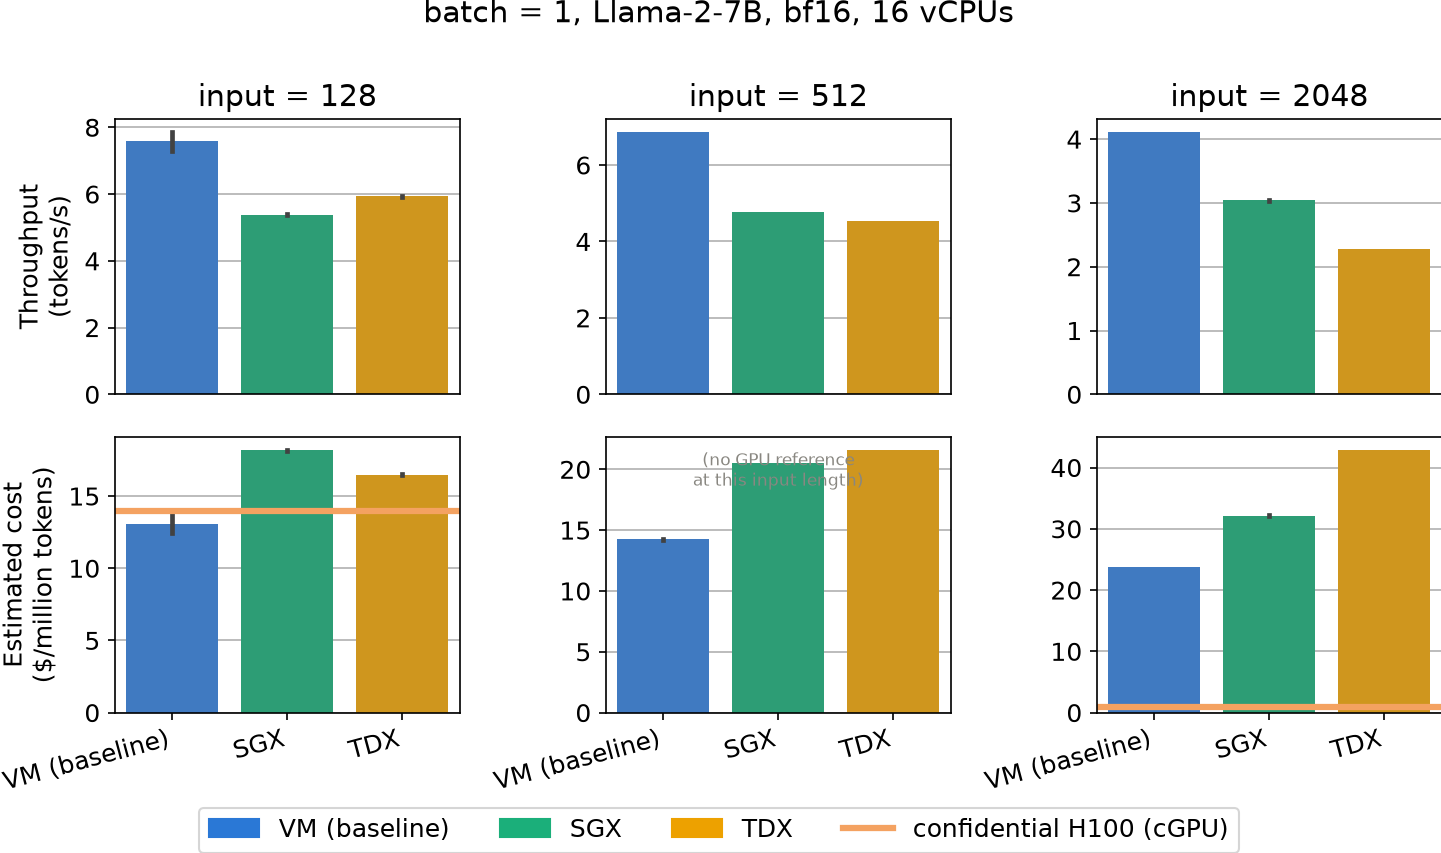
\includegraphics[width=0.85\textwidth]{vCPUs_GPU_EMR_inputs.png}
  \caption{Measured throughput (top) and estimated cost per million generated tokens
  (bottom) at batch size 1, by input length, using the same cost model as
  Figure~\ref{fig:cost-batches}.}
  \label{fig:cost-inputs}
\end{figure*}

Figures~\ref{fig:cost-batches} and~\ref{fig:cost-inputs} combine the measured
throughput with the original artifact's cost model to estimate the cost of generating
one million tokens in each environment; Figure~\ref{fig:azure-price} shows the
pricing efficiency of the two VM families, for context on the price asymmetry between
the SGX- and TDX-capable instances. \textbf{[PLACEHOLDER --- cost interpretation]}
Once finalized, this paragraph will discuss whether CPU TEEs remain cost-competitive
with the confidential-GPU reference at low batch sizes, as claimed by the original
study.

\subsection{Key Findings}
\label{sec:key-findings}

\textbf{[PLACEHOLDER --- to be completed once data collection finishes]}
\begin{itemize}
  \item \textbf{RQ1:} TBD --- whether the $<$10\% throughput overhead bound holds for
  both SGX and TDX on independent hardware.
  \item \textbf{RQ2:} TBD --- whether relative overhead diminishes with larger batch
  sizes and longer input sequences, consistent with the original study.
\end{itemize}

% ---------------------------------------------------------------
\section{Threats to Validity}
\label{sec:threats}

\textbf{Internal validity.} Measurements are taken on shared cloud/virtualized
infrastructure (Scontain or Microsoft Azure), so noisy-neighbor effects from co-located
tenants and CPU frequency/turbo-boost variability across repetitions could inflate
variance independent of the TEE mechanism under test. This is mitigated by taking 30
repetitions per configuration and reporting medians, and by pinning all environments to
the same Docker image (\texttt{ipex-llm:2.3.100}) and the same 16-vCPU core binding, so
that software version drift does not confound the environment factor.

\textbf{External validity.} The reproduction hardware (a 16-vCPU, 64\,GB VM on Scontain
or Azure) differs from the original study's Intel Xeon Gold 6530 and Platinum 8580
server platforms, which may have different SGX EPC sizes, TDX virtualization stacks, and
AMX/AVX-512 microarchitectural behavior even with AMX disabled. The factor space is also
narrower than the original study's, as summarized in Table~\ref{tab:differences}: only
Llama2 7B is evaluated (no 13B/70B, Llama3, Mistral, or Gemma), no bare-metal baseline is
included, and GPU TEEs are out of scope. Conclusions drawn here therefore generalize to
this specific model size and hardware class, not to the full space covered by the
original study.

\textbf{Construct validity.} Throughput and next-token latency are used as proxies for
``performance overhead,'' following the original study's definition; reporting only
medians across 30 repetitions may obscure tail-latency behavior that matters for
latency-sensitive deployments. The synthetic, fixed-length workloads (128/512/2048 input
tokens, 128 output tokens, greedy decoding) may not reflect the input-length
distribution or decoding strategy of production LLM serving traffic.

\textbf{Conclusion validity.} \textbf{[PLACEHOLDER]} This paragraph will state whether
overhead differences between environments are assessed with a formal statistical test
(e.g., a non-parametric test across the 30 repetitions) or only via descriptive medians;
if the latter, that is noted here as a limitation on the strength of the RQ1/RQ2
conclusions.

% ---------------------------------------------------------------
\section{Conclusion}
\label{sec:conclusion}

This paper set out to reproduce the CPU TEE performance evaluation of
Chrapek et al.~\cite{chrapek2025confidential} on hardware independent from the original
study, comparing Intel SGX (via Gramine) and Intel TDX against a conventional VM
baseline for Llama2 7B inference across a range of batch sizes and input lengths.
\textbf{[PLACEHOLDER --- RQ verdict]} Once the measurement matrix in
Section~\ref{sec:results} is complete, this paragraph will state whether RQ1's $<$10\%
throughput overhead bound and RQ2's overhead-amortization trend hold on independent
hardware, and will discuss the implications for practitioners deciding between SGX- and
TDX-based confidential LLM deployments.

Beyond the specific overhead figures, this reproduction contributes an independent data
point on the hardware-sensitivity of confidential-computing performance claims for LLM
inference --- a question of practical importance given how frequently such workloads are
deployed on infrastructure the original researchers never had access to. Future work
includes extending this reproduction to the GPU TEE scenario (NVIDIA H100 confidential
computing) and to larger model sizes (13B, 70B), both left out of the present scope for
resource reasons (Table~\ref{tab:differences}).

% ---------------------------------------------------------------
\section{Reproducibility}
\label{sec:reproducibility}

All artifacts of this reproduction are public in a fork of the original study's
repository:
\begin{center}
  \url{https://github.com/raissonsouto/confidential-llms-in-tees} (branch \texttt{develop})
\end{center}
% TODO: add the Zenodo/OSF DOI of the archived snapshot once minted.

\textbf{What is available.} The fork contains (i) the benchmark scripts and the
patches applied on top of the original artifact, with the third-party dependencies
(IPEX, Gramine, Canonical TDX tooling) pinned as submodules; (ii) \texttt{AZURE.md},
a step-by-step runbook to provision the cloud infrastructure; (iii) the top-level
\texttt{README.md} with the end-to-end experiment instructions; and (iv) the
\texttt{results/} directory with the raw benchmark logs of every arm (one folder
per arm, including \texttt{lscpu}, \texttt{lshw}, and \texttt{numactl}
hardware snapshots), the consolidated \texttt{results.csv} with per-iteration
latencies generated by \texttt{CPU/processing/run\_parser.py}, and the figures of
Section~\ref{sec:results} together with the plotting scripts
(\texttt{CPU/processing/}) that produce them. The \LaTeX{} source of this paper is
in \texttt{paper/}. Runs that failed
(e.g., out-of-memory at batch~64 with long inputs) are published as-is, since the
failure modes are themselves findings.

\textbf{How to reproduce.} (1)~Provision the two VMs following \texttt{AZURE.md};
(2)~on each VM, follow the \texttt{README.md} common setup (clone, initialize
submodules, apply patches, run \texttt{host\_setup.sh}, and build the Docker image);
(3)~run the baseline and TDX arms with \texttt{./run.sh baseline} and
\texttt{./run.sh tdx}, and the SGX arm with \texttt{sgx\_setup.sh} followed by
\texttt{run\_sgx\_sweep.sh} (from \texttt{CPU/}); (4)~parse the logs with
\texttt{run\_parser.py} to obtain the CSV used in the analysis.

\textbf{Required resources.} Two Azure VMs: \texttt{Standard\_DC16s\_v3}
(16~vCPUs, 128\,GB, Ice Lake; hosts the baseline and SGX arms) and
\texttt{Standard\_DC16es\_v6} (16~vCPUs, 64\,GB, Emerald Rapids; hosts the TDX arm),
both on Ubuntu 24.04 with a 128\,GB OS disk. Provisioning requires vCPU quota for
the \texttt{DCSv3} and \texttt{DCESv6} families (default quota is zero on new
subscriptions) and a Hugging Face token with the Llama-2 license accepted. At
roughly US\$1.5--2 per VM-hour, one full sweep per arm takes several hours,
dominated by the batch-64 configurations.

% ---------------------------------------------------------------
\section*{AI Usage Disclosure}

The author used Claude Code (Claude, Anthropic) as an assistant throughout this
project: diagnosing and patching the original artifact's build and benchmark
scripts, drafting the provisioning runbook, analyzing benchmark logs, generating
the consolidated results CSV, and revising the documentation and the \LaTeX{}
source of this paper. All experimental design decisions, the execution of the
experiments, and the validation of results and text remain the author's; the
author reviewed all AI-assisted output and takes full responsibility for the
content of this paper and its artifacts.

% ---------------------------------------------------------------
\bibliographystyle{ACM-Reference-Format}
\bibliography{references}

\end{document}
